\chapter{Methodology}\label{ch:methodology}

This chapter outlines the methodological approach taken to bridge the identified gaps between values-driven impact measurement and practical, scalable tools supported by artificial intelligence.
Grounded in the context of the Public Value Hub in Leipzig, this research combines qualitative inquiry with experimental AI applications to explore how language models can support meaning-making in public innovation.

\section{Research Design}\label{sec:research-design}

The study follows a mixed-methods, exploratory design, combining:

\begin{itemize}
    \item Qualitative research, including semi-structured stakeholder interviews and participatory workshops, to identify core needs and values in public sector impact work.
    \item Experimental development of AI-supported tools, specifically using large language models (LLMs) for natural language understanding and semantic analysis.
\end{itemize}

The overall approach is informed by design science and action research traditions, aimed at producing both understanding and actionable prototypes in a real-world innovation setting.

\section{Qualitative Inquiry}\label{sec:qualitative-inquiry}

Interviews were conducted with public sector innovators and researchers affiliated with the Public Value Hub and the Public Value Academy.
These engagements explored:

\begin{itemize}
    \item Current impact measurement challenges in innovation projects,
    \item How concepts like \textbf{public value} are interpreted in practice,
    \item Stakeholder needs for sense-making, learning, and transparency in evaluation.
\end{itemize}

Thematic analysis of transcripts was used to extract design criteria for the AI components — particularly around interpretability, flexibility, and the need to reflect both quantitative and narrative dimensions of impact.

\section{LLM-Based Tool Development}\label{sec:llm-based-tool-development}

This section describes the development of AI-supported tools designed to augment — not automate — value-driven decision-making in public innovation.

\subsection{Narrative Analysis of Pitch Decks}\label{subsec:narrative-analysis-of-pitch-decks}

To support early-stage project evaluation, pitch decks from public innovation teams were analyzed using an LLM (e.g., OpenAI’s GPT-4).
The model was prompted to extract:

\begin{itemize}
    \item Key impact themes,
    \item Evidence of alignment with public value dimensions,
    \item Indicators of potential long-term benefit or stakeholder inclusion.
\end{itemize}

Outputs were compared across cases to test for consistency and relevance, serving as a prototype for narrative-based impact reviews.

\subsection{Semantic Similarity Search Across Frameworks}\label{subsec:semantic-similarity-search-across-frameworks}

A corpus of over 40 different evaluation frameworks, sourced from academia, government, and practice, was compiled and pre-processed.
The goal was to support innovation teams in selecting or aligning with existing approaches.

Using sentence embeddings (via BERT or Sentence-Transformers), a similarity search tool was built to allow users to query their own impact statements or goals against this corpus to discover:

\begin{itemize}
    \item Conceptual overlaps,
    \item Implicit values in each framework,
    \item Alternative metrics or lenses for evaluation.
\end{itemize}

This addressed a recurring concern in interviews: that existing frameworks are often applied blindly or bureaucratically, without being interrogated for fit or value alignment.

\subsection{Clustering and Thematic Grouping of Narratives}\label{subsec:clustering-and-thematic-grouping-of-narratives}

To identify recurring themes in unstructured narratives emerging from public innovation contexts — such as project proposals, workshop transcripts, or citizen inputs — a semantic clustering pipeline was implemented.
The goal was to surface latent topics reflecting common challenges, priorities, or value framings across diverse projects.

\textbf{Embedding Generation:} Narrative inputs were converted into dense vector representations using OpenAI’s \texttt{text-embedding-ada-002} model~\parencite{OpenAI2023Embedding}, selected for its ability to capture rich semantic relationships beyond surface lexical similarity~\parencite{Reimers2019SentenceBERT}.

\textbf{Dimensionality Reduction:} To reduce noise and improve interpretability, embeddings were optionally projected into a lower-dimensional space using Uniform Manifold Approximation and Projection (UMAP)~\parencite{McInnes2018UMAP}, which preserves local and global data structure better than PCA~\parencite{vanDerMaaten2008tSNE}.

\textbf{Clustering:} Hierarchical Density-Based Spatial Clustering of Applications with Noise (HDBSCAN)~\parencite{Campello2013HDBSCAN} was employed, which suits variable-density clusters and noisy data typical in qualitative text corpora.

\textbf{Cluster Interpretation:} Representative documents from each cluster were summarized using GPT-4~\parencite{OpenAI2023GPT4} to generate interpretable labels, leveraging advances in large language models for thematic summarization~\parencite{Bamman2020LLMTextMining}.

\textbf{Use in Downstream Tasks:} Thematic clusters informed subsequent pipeline stages such as KPI generation, and facilitated stakeholder reporting by providing structured overviews of diverse narrative inputs, enhancing transparency and reflection~\citep{Braun2019ThematicAnalysis,Feng2019MixedMethodsNLP}.


\begin{figure}[H]
    \centering
    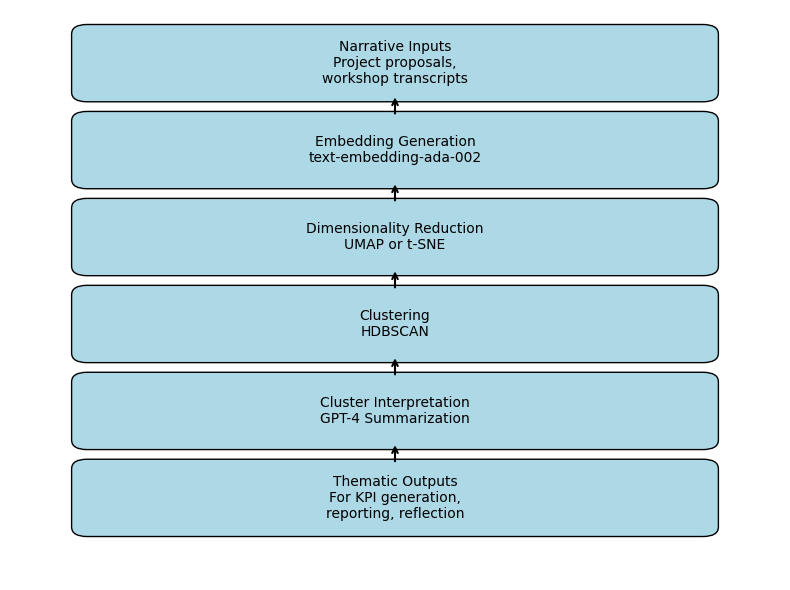
\includegraphics[width=0.9\textwidth]{../fig/clustering_pipeline}
    \caption{Semantic Clustering Pipeline for Narrative Inputs}
    \label{fig:clustering-pipeline}
\end{figure}

% Continue with text referencing Figure~\ref{fig:clustering-pipeline}

\subsection{Automated KPI Derivation via LangGraph Pipelines}\label{subsec:kpi-pipeline}

To explore how generative AI can support structured evaluation in public innovation, a modular pipeline was developed using the LangGraph framework — a tool for orchestrating large language models in stateful workflows.
The objective was to generate context-sensitive, auditable Key Performance Indicators (KPIs) based on unstructured or semi-structured problem descriptions, reflecting relevant dimensions of public value and providing measurable evaluation anchors.

The pipeline stages included:

\begin{enumerate}
    \item \textbf{Input normalization:} Raw problem statements (e.g., from project proposals or workshop materials) were structured into a consistent format including scope, context, and constraints.
    \item \textbf{SDG Mapping:} Using a GPT-4-based classifier, each problem was aligned to one or more Sustainable Development Goals (SDGs) through semantic understanding rather than keyword matching.
    \item \textbf{Audit Loop 1 — SDG Justification:} A second language model performed rationale-based auditing of the SDG classification to ensure plausibility and provide explanatory feedback.
    \item \textbf{Indicator Retrieval:} Vector similarity search (via FAISS or pgvector) was used to identify candidate indicators from a curated global indicator database relevant to the problem context.
    \item \textbf{Audit Loop 2 — Indicator Fit:} A critic model re-evaluated indicators for semantic and practical fit, discarding weak matches and refining selection criteria.
    \item \textbf{KPI Generation:} Tailored KPIs were proposed based on selected indicators and contextual cues, including name, definition, measurement logic, and suggested targets or baselines.
    \item \textbf{Audit Loop 3 — KPI Quality:} KPIs were scored using a rubric assessing clarity, measurability, and context alignment.
    \item If quality was insufficient, regeneration was triggered.
    \item \textbf{Optional — Transparency Trace:} An explanatory trace of the KPI generation process was produced for interpretability, outlining key steps and reasoning behind outputs.
\end{enumerate}

The LangGraph framework was chosen for its support of branching logic, audit loops, and modular AI-driven tasks — enabling reflexive, explainable tool development rather than rigid automation.
The pipeline was tested with synthetic and anonymized project descriptions from public innovation settings, demonstrating potential to offer structured, explainable KPIs aligned with broader value narratives.

\begin{figure}[H]
    \centering
    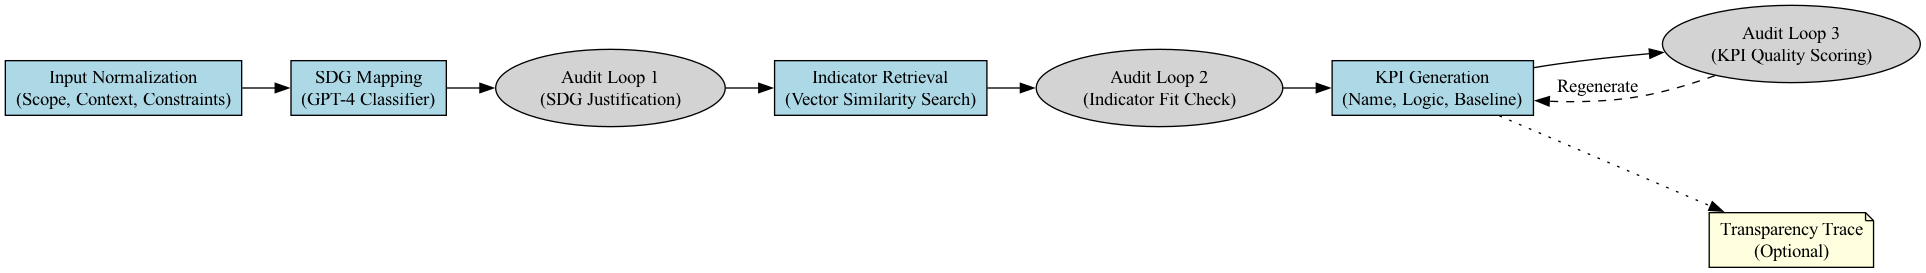
\includegraphics[width=0.9\textwidth]{../fig/langgraph_pipeline}
    \caption{Langgraph pipeline}
    \label{fig:langgraph-pipeline}
\end{figure}

\section{Integration into Public Value Academy Platform}\label{sec:integration-into-public-value-academy-platform}

To test applicability, these AI tools were designed for compatibility with the existing Public Value Academy digital infrastructure.
This platform supports workshops and guided reflection around public value and innovation — making it a suitable space to prototype and iteratively improve language-based evaluative tools.

\section{Evaluation Strategy}\label{sec:evaluation-strategy}

Given the exploratory nature of this work, a formative evaluation approach was adopted.
Tools were tested using anonymized project documents, workshop materials, and synthetic inputs.
Early feedback was gathered through user walkthroughs and informal interviews with practitioners and researchers.

Evaluation criteria included:

\begin{itemize}
    \item Usefulness and clarity of AI-generated insights,
    \item Perceived alignment with stakeholder values and expectations,
    \item Potential for embedding in existing impact workflows without undermining deliberation.
\end{itemize}

\section{Ethical Considerations}\label{sec:ethical-considerations}

All qualitative research participants provided informed consent, and data was handled in accordance with GDPR and academic ethical guidelines.
AI components were designed to promote interpretability and reflection — avoiding prescriptive or opaque outputs.
This reflects the project's core principle that computational tools serve as aids to human judgment, not substitutes for ethical deliberation or political accountability.